

\newpage
\section{Design and Implementation}
This section will be discussing the main contribution of this project: a implementation of lattice Boltzmann method on SpiNNaker.  \\

All the source code is available at: \url{https://github.com/YuaNFrank/SpiNN_LB}.
\subsection{Implementation Overview}

As we discussed at \ref{sec:sdw}, in general SpiNNaker development workflow, the first thing we did is to define the computation graph in Python. We will discuss how we define the lattice vertex (\ref{sec:tlc}), how we define our edge (\ref{sec:tle}), and how we connect them together as a graph (\ref{sec:tcg}). All these steps are implemented in Python API.

Then on the computation side, as discussed at \ref{sec:lbmb}, there are five step for a lattice Boltzmann method in general. While the first four steps do not involve communication, and can be calculate locally for each lattice vertex (discussed at \ref{sec:cp}), the last step, the streaming step, is where the communication happens, which we will focus on at \ref{sec:ssc}. These computation-wise code is written in C.

\subsection{The Lattice Cell} \label{sec:tlc}
\subsubsection{Design Consideration} \label{sec:tlcdc}
In the lattice cell class, we will define the data regions needed for simulation. In implementation, it need to acquire those data, reserve memory for the data and pass the data in SpiNNaker SDRAM in Python, then define how to read the data from the SDRAM during simulation in C. The data regions that a lattice might need for simulation are: \\

\begin{itemize}
    \item \textbf{System Information:} for every simulation, they at least need some memory reserved for the runtime system such as the how long is a machine time step. And the developers need to generate the system data region and allocate memory for them manually.
    
    \item \textbf{Transmission Information:} for non-embarrassingly parallel problems, the simulation are involved in communication. The keys are generated by the runtime, and the developers can ask the runtime for a fix number of keys for every lattice. The developers need to allocate memory for the transmission keys and pass the keys to the cores, correspondingly.

    \item \textbf{Position Information:} in lattice Boltzmann, a lattice might need to know what is its position \textbf{(x,y)} among the whole simulation lattices. The position information would be generated when connecting the lattices as a graph, and then pass them into the application.
    
    \item \textbf{Initialized Velocity:} in lattice Boltzmann method, the velocity need to be generated according to the specific problem. We can either initialize it in Python then pass then in or initialize it in the simulation according to the position. A more detailed discussion is at \ref{sec:ip}.
    
    \item \textbf{Routing Information of Neighbours:} in lattice Boltzmann method, the lattice need to exchange the momentum and energy by moving the distribution function with its eight neighbours. This involve a few communication and the lattice need to know which are its eight neighbours and their routing information i.e. routing keys to communicate with them. Thus allocating memory and pass them into the cores is necessary. 
    
    \item \textbf{Index of this Lattice:} we might need to know the index of the lattice in the whole simulation fabric. This might not be necessary for a simple prototype. Since the random number generation is relatively slow, we can use it as a random number in practice. A further discuss is at \ref{sec:ssc}.
    
    \item \textbf{Result Recording:} the SDRAM in SpiNNaker is relatively limited (\ref{sec:sa}). We can use the recorded data to store larger simulation result more reliably. We can specify the an area of memory used for recording the results and get them back when the simulation ends.
\end{itemize}

\subsubsection{Final Implementation}
In the final implementation, we defined the discussed data regions in the \textit{LatticeBasicCell} class following the pattern: get the data; allocate memory; write the data in. For different data, there are different way to get the data:

\begin{itemize}
    \item \textbf{System Information:} the \textit{SpiNNaker GraphFrontEnd} provide API to generate the system data region.
    \item \textbf{Transmission Information:} the SpiNNaker runtime would allocate keys for the cores.
    \item \textbf{Position Information:} the position information is decided during runtime. it will be passed as class variables.
    \item \textbf{Initialized Velocity:} the velocities are decided during runtime with a initialization function. They will be passed as class variables. 
    \item \textbf{Routing Information of Neighbours:} a lattice can know the which are its neighbours by asking the connected edges. We will illustrate how we implement it at \ref{sec:tle}. After knowing its neighbours, we can get their routing keys via the get\_routing\_info\_from\_pre\_vertex() function from the \textbf{PACMAN} library.
    \item \textbf{Index of Lattice:} we can ask the graph system for the index of a lattice.
    \item \textbf{Result Recording:} we do not need to get data from result recording since it is for the result.
\end{itemize}

After all the data are acquired, we get then reserve corresponding memory and write the data into the SDRAM of each SpiNNaker core; see code code block \ref{lst:code1}. Correspondingly, in the C file, we also need to get the data from the SDRAM; see code block \ref{lst:code2}. The \ref{lst:general} shows a piece of code from our final implementation on how to reserve memory for the position data and write the data into the SDRAM followed by how to read the written data from the SDRAM during simulation in C.

\begin{figure}[!ht]
\setcounter{tmp}{\thefigure}
\setcounter{figure}{\thelstlisting}
\captionsetup{list=no,name=Listing}
\begin{subfigure}{\linewidth}
\begin{lstlisting}
# spec is the handle for data specification API
# reserve memory for a data region, POSITION, with a size, POSITION_DATA_SIZE
spec.reserve_memory_region(
            region=self.DATA_REGIONS.POSITION.value,
            size=self.POSITION_DATA_SIZE, label="position")

# switch the cursor to the data region of REGION
spec.switch_write_focus(
            region=self.DATA_REGIONS.POSITION.value
        )
# write the position data (x,y) in the device 
spec.write_value(int(self.x_position))
spec.write_value(int(self.y_position))
\end{lstlisting}
\caption{An example of how to reserve memory for the position data region and write data to the device in Python.\\}
\label{lst:code1}
\end{subfigure}
\begin{subfigure}{\linewidth}
\begin{lstlisting}
// get the address starting the DTCM from the SRAM on this SpiNNaker core
data = data_specification_get_data_address();

// get position data from the DTCM
position_data_t position_data = data_specification_get_region(POSITION, data);
\end{lstlisting}
\caption{An example of how to read the position data in C.}
\label{lst:code2}
\end{subfigure}
\caption{An exmaple of how to pass the position data to SpiNNaker.}
\label{lst:general}
\addcontentsline{lol}{lstlisting}{\protect\numberlineAn example of how to pass the position data to SpiNNaker.}
\stepcounter{lstlisting}
\setcounter{figure}{\thetmp}
\end{figure}


\subsection{The Lattice Edge} \label{sec:tle}
\subsubsection{Design Consideration}
The major job of the lattice edge except connecting two lattice cells is providing a way that the lattice cell can get the vertex on the other end of this edge in a given direction. So that each lattice can get the routing information (routing keys) of its eight neighbours with knowing the direction. 
\subsubsection{Final Implementation}
\begin{figure}[!tb]
   \centering
       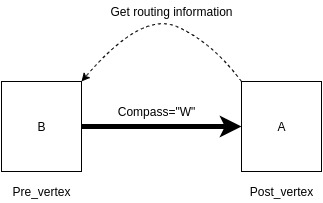
\includegraphics[width=0.8\textwidth]{figures/edge.jpg}
       \caption{A lattice cell A connected by another lattice B via a lattice edge with the compass being "W". The lattice A then can get the routing key from its pre\_vertex, B.}
       \label{fig:edge}
\end{figure}

\subsection{The Computational Graph} \label{sec:tcg} %TODO: a comparison between the spinnaker computational graph and the lattice boltzmann boundary condition
\subsubsection{Design Consideration}
\subsubsection{Final Implementation}


\subsection{Initialize Parameters} \label{sec:ip}
\subsubsection{Design Consideration}
To initialize the parameters for the lattice Boltzmann, there are two different way in general. The first one is initialization on host (in Python), and the other one is initialization on SpiNNaker (in C).
\subsubsection{Final Implementation}

\subsection{Computation Implementation} \label{sec:cp}
\subsubsection{Design Consideration}
\subsubsection{Final Implementation}

\subsection{Streaming Step -- Communication Implementation} \label{sec:ssc}
\subsubsection{Design Consideration}
\subsubsection{Final Implementation}